\documentclass[a4paper,ngerman]{atseminar}

\usepackage{microtype}
\usepackage{graphicx}
\usepackage{algorithm2e}
\usepackage[left]{lineno}
\linenumbers

%% Please do not include packages that change the layout/size of the
%% of the document. They will be removed.

\bibliographystyle{plain}%the recommended bibstyle

% Preamble with header information 
\subject{Ausarbeitungen für das Proseminar}
\title{Algorithmen für NP-schwere Probleme}
\titlerunning{Proseminar Algorithmen für NP-schwere Probleme}%optional





%Organizer macros:%%%%%%%%%%%%%%%%%%%%%%%%%%%%%%%%%%%%%%%%%%%%%%%%%%%%%


%% do not use this field, but \summaryauthor
\author{}

%%%%%%%%%%%%%%%%%%%%%%%%%%%%%%%%%%%%%%%%%%%%%%%%%%%%%%%%%%%%%%%%%%%%%%%%%%%%%%%
%%%%%%%%%%%%%%%%%%%%%%%% begin of document %%%%%%%%%%%%%%%%%%%%%%%%%%%%%%%%%%%%
%%%%%%%%%%%%%%%%%%%%%%%%%%%%%%%%%%%%%%%%%%%%%%%%%%%%%%%%%%%%%%%%%%%%%%%%%%%%%%%
\begin{document}

\maketitle

\GERMAN

%%%%% YOUR REPORT BEGINS HERE
\section{Titel der Ausarbeitung}
\summaryauthor[Dein Name]{Dein Name}

\begin{abstract}
Eine kurze Zusammenfassung der Ausarbeitung. 
\end{abstract}

Hier steht der Inhalt der Ausarbeitung.



\subsection{Abschnitt der Ausarbeitung}

\subsubsection{Unterabschnitt der Ausarbeitung}


\paragraph{Bitte keine Paragraphen verwenden!}


\begin{figure}[h]
 \centering
 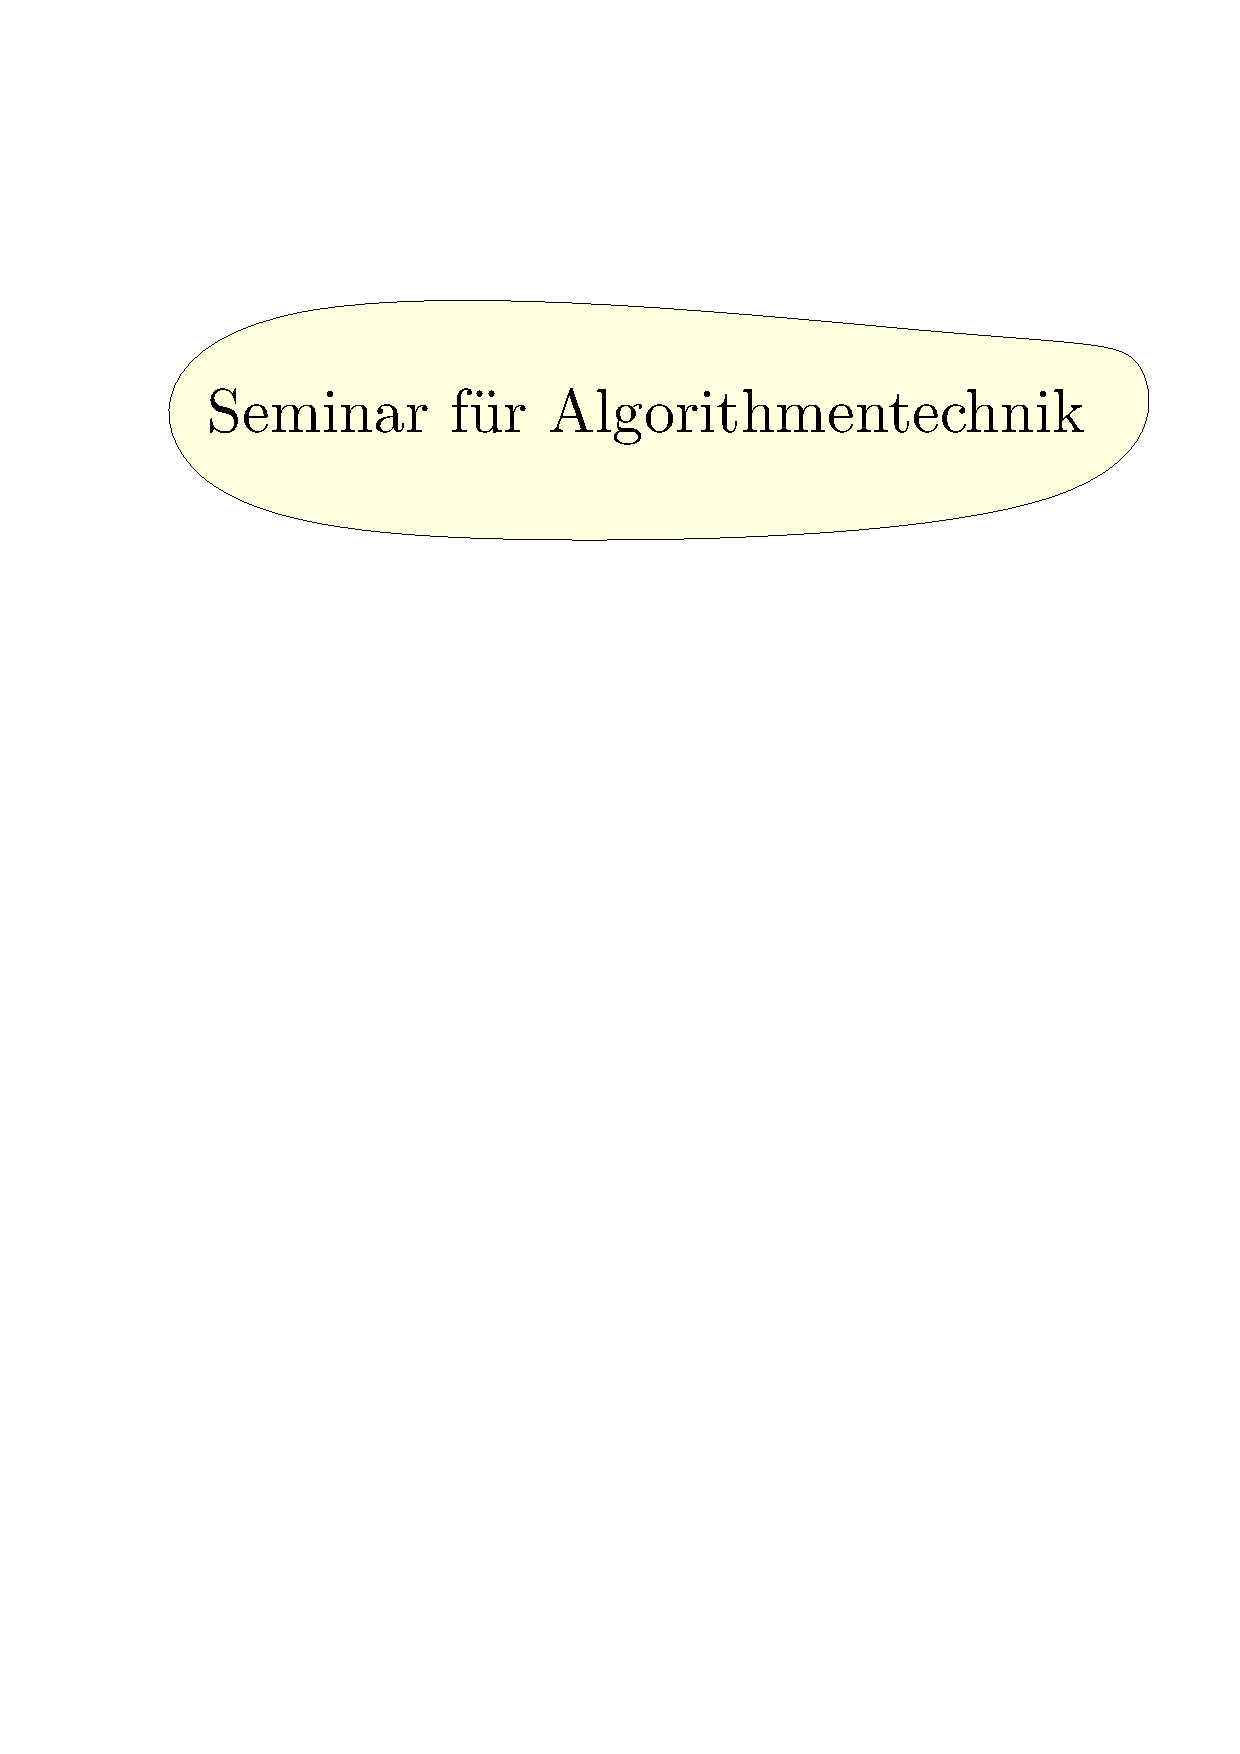
\includegraphics[scale = 0.7]{./picture}
 \caption{Dies ist die Beschreibung der Abbildung: Kurze Erklärung
was zu sehen ist.}
 \label{XY:fig:picture}
 % where X is the first letter of your first name and Y is the
% first letter of your last name.
\end{figure}

\begin{table}[h]
\centering
\caption{Tabellen haben Überschriften.}
\begin{tabular}{l|ll}
  \textbf{Zelle11} & \textbf{Zelle12} & \textbf{Zelle13} \\
  \hline
  \textbf{Zelle21} & Zelle22 & Zelle23 \\
  \textbf{Zelle31} & Zelle32 & Zelle33 \\
  
\end{tabular}
\label{XY:tab:interessant}
% where X is the first letter of your first name and Y is the
% first letter of your last name.
\end{table}



\begin{algorithm}[H]
\caption{Greedy}
\KwIn{Menge $\mathcal{C}$ aller Kreise in $G=(V,E)$.}
\KwOut{ Kreisbasis minimalen Gewichts von $G$.}
Sortiere $\mathcal{C}$ aufsteigend nach Gewicht zu $C_1,\ldots,C_k$\; 
$\mathcal{B}^\star$ $\leftarrow$ $\emptyset$\; %
  \For{$i = 1$ \KwTo $k$}{ %
    \If{$\mathcal{B}^\star \cup \{C_i\}$ linear unabhängig}{ %
      $B^\star$ $\leftarrow$ $B^\star \cup \{C_i\}$\; 
    }
} %
\end{algorithm}

\begin{theorem}[Titel des Theorems (optional)]
 Die Aussage des Theorems.
\end{theorem}

\begin{proof}
 Der Beweis für das Theorem.
\end{proof}

\begin{example}
 Dies ist ein Beispiel.
\end{example}


\begin{lemma}[Titel des Lemmas (optional)]
 Die Aussage des Lemmas
\end{lemma}

\begin{corollary}[Titel des Korollar (optional)]
 Ein Korollar.
\end{corollary}


\begin{definition}[Titel der Definition(optional)]
Inhalt der Definition
\end{definition}

Das erste Beispiel \cite{example1}, das zweite Beispiel
\cite{example2} und  das dritte Beispiel \cite{example3, example4}
für eine Referenz.

\subsection{Zweiter Abschnitt}


\begin{definition}[Titel der Definition(optional)]
Inhalt der Definition
\end{definition}





\bibliography{references}



%%%%% YOUR REPORT ENDS HERE




\end{document}
